\section{Before Getting Started}
\label{tutorial_01}

Before we get started with the actual tutorial, we are going to go over the required background to make sure that you have a rudimentary understanding of the necessary concepts.

\tick{\textbf{You can skip this section, if...}
\begin{itemize}
	\item ... you a familiar with \bms
	\item ... you know what formal modelling is
	\item ... you know what predicate logic is
	\item ... you know what ProB refer to
\end{itemize}
}

\subsection{BMotion Studio}

\begin{figure}[!ht]
\begin{center}
	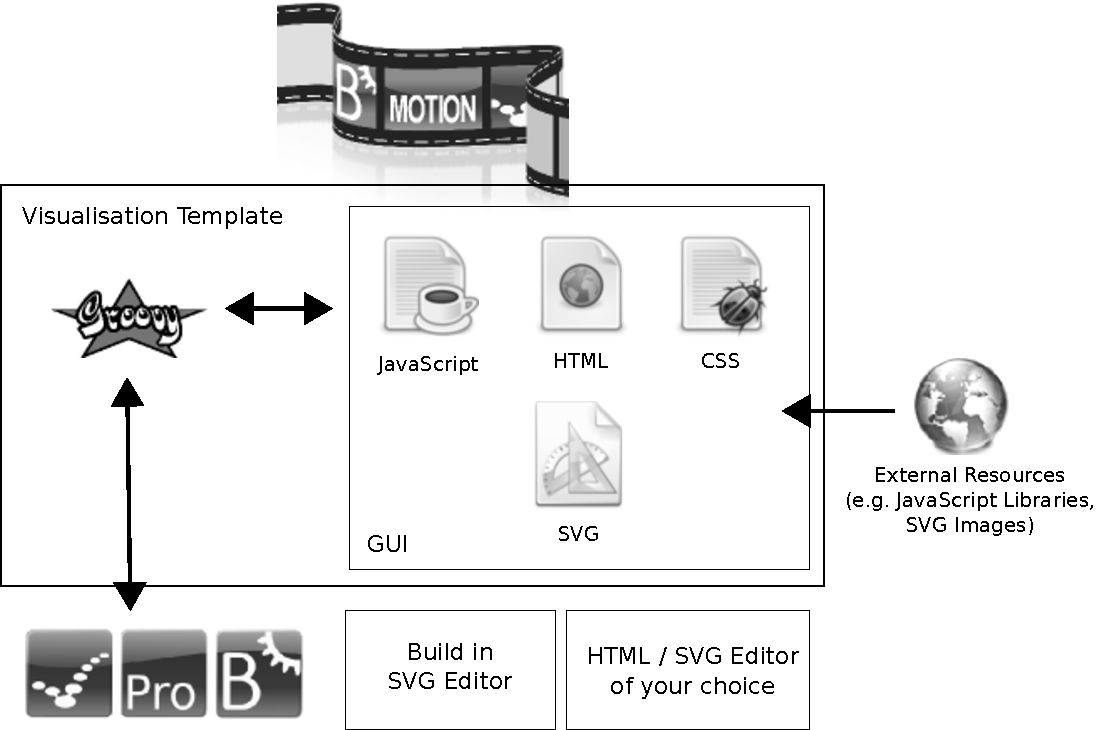
\includegraphics[width=14cm]{img/tutorial/bms_architecture}
	\caption{\bms~Architecture}
	\label{fig_tut_00_architecture}
\end{center}
\end{figure}

Figure~\ref{fig_tut_00_architecture} shows an overview of the architecture of \bms. 
In \bms, a visualisation is described by a visualisation template that contains visual elements and observers. 
Visual elements may be, for instance, shapes or images that represent some aspects of the model. 
For example, when modelling a communication protocol, circles may be used for representing the communicating entities of the protocol and arrows for the message exchanges between the entities. 
\bms~supports web technologies like Scalable Vector Graphics (SVG)\footnote{\url{http://www.w3.org/TR/SVG11}} and Cascading Style Sheets (CSS)\footnote{\url{http://www.w3.org/TR/css-2010}} for this purpose. 
SVG is an XML-based markup language for describing two-dimensional vector graphics. 
It comes with a number of visual elements like shapes, images and paths.
CSS is a language that can be used to describe the style of SVG visual elements (e.g. the colour or the dimension). 

Observers are used to link visual elements with the model. 
An observer is notified whenever a model has changed its state, i.e. whenever an event has been executed. 
In response, the observer will query the model's state and triggers actions on the linked visual elements in respect to the new state. 

\subsection{Formal Modelling}

We are concerned with \textit{formalizing specifications}.  This allows us a more rigorous analysis (thereby improving the quality) and allows the reuse of the specification to develop an implementation.  This comes at the cost of higher up-front investments.

This differs from the traditional development process. In a formal development, we transfer some effort from the test phase (where the implementation is verified) to the specification phase (where the specification in relation to the requirements is verified).

\subsection{Predicate Logic}
\label{predicate_logic}
\index{predicate logic}

Predicate logic is a mathematical logic containing variables that can be quantified.

Event-B supports first-order logic which is, technically speaking, just one type of predicate logic.  

\subsection{Event-B}
\label{eventb}
\index{Event-B}

Event-B is a notation for formal modelling based around an abstract machine notation (\index{abstract machine notation}).

Event-B is considered an evolution of B (also known as Classical B). It is a simpler notation which is easier to learn and use. It comes with tool support in the form of the Rodin Platform.

\subsection{ProB Animator}
\label{prob_animator}

ProB is a validation toolset for the B method including an animator, a modelchecker and other useful tools to allow users to gain confidence in their specifications. One of the components of ProB is animation. The animation component allows the user to check the presence of desired functionality and to inspect the behaviour of a specification by "clicking through" the states of the specification. ProB also provides other useful tools such as a tool to visualize graphically any predicate as a tree or a tool for graphical state representation. Such tools, especially the tool for the graphical state representation can give a better understanding of the model.
